\chapter{Global Supercoiling in \emph{Aevol}}
\label{chap:aevol}

In this chapter, I present the first main line of work of that I undertook during my Ph. D., in which I implemented a model of the effect of DNA supercoiling on gene transcription into the \emph{Aevol} \emph{in silico} experimental evolution platform, in order to study the possible epistatic interactions between mutations that regulate the supercoiling level and other kinds of mutations.

\section{Introduction}
\label{sec:aevol:intro}

In the \emph{Long-Term Evolution Experiment}, started by Richard Lenski in 1988~\citep{lenski1991}, 12 populations of \emph{E. coli}, originating from the same ancestral strain, were placed to evolve in a new environment, a glucose-limited medium.
Every day since the beginning of the experiment, which is still running, a sample from each population has been propagated into fresh medium, resulting in the longest-running evolution experiment in the lab, and demonstrated that fitness can keep on increasing for much longer than originally expected in a constant environment~\citep{good2017}.
As sequencing capacity and synthetic biology developed in the late 1990s and early 2000s, identifying the precise DNA mutations underpinning these increases in fitness became possible.
Mutations in the \emph{fis} and \emph{topA} gene were thus found to lead to an increased growth rate in the conditions of the experiment, as well as to an increase in the basal supercoiling level of the cells bearing these mutations~\citep{crozat2005}.
\textbf{Devrait plutôt aller dans l'intro globale ?
Tel quel ça pose la question du rôle de la superhélicité dans l'évolution mais il n'y a pas (dans Crozat 2005 ou 2010) d'étude des suites évolutives de ces mutations de superhélicité.}

As mutations in genes regulating the level of supercoiling in \emph{E. coli}, such as \emph{topA} and \emph{fis}, were shown to increase fitness in the LTEE, we sought to investigate whether these mutations, by globally altering the regulatory landscape of the cell, could open up new evolutionary pathways and thereby speed up evolution, that is display positive epistasis with other mutations.
In order to explore this theoretical possibility without having to resort to wet-lab experiments, I resorted to the \emph{in silico} experimental evolution toolbox, using the \emph{Aevol} platform.


\section{The \emph{Aevol} model}
\label{sec:aevol:model}

\begin{figure}[H]
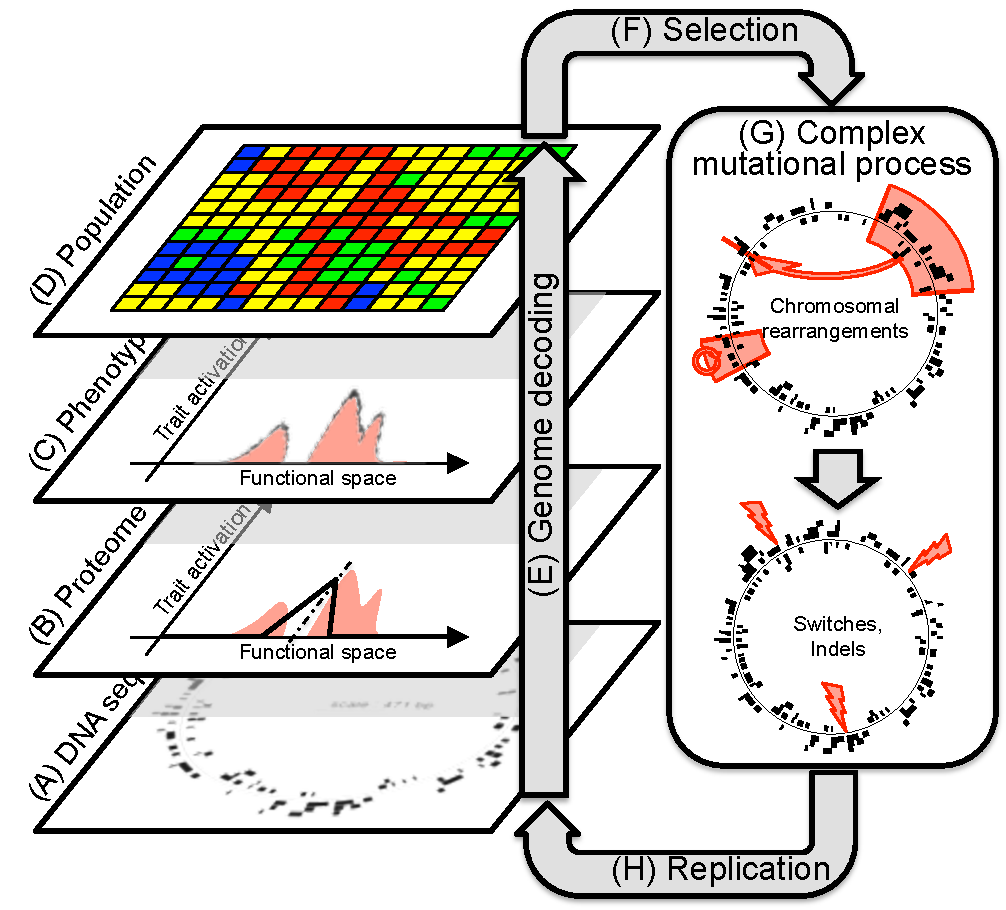
\includegraphics[width=\textwidth]{aevol/images/aevol.pdf}
\caption[Overview of the \emph{Aevol} model]{Broad overview of the \emph{Aevol} model.}
\label{fig:aevol:model}
\end{figure}

\subsection{Overview}

The \emph{Aevol} platform, developed in the Inria Beagle team~\citep{rutten2019}, is a software suite designed to run artificial evolution experiments on a computer, rather than at the bench.
As an excellent and very thorough description of \emph{Aevol} (in French) can be found in~\cite{liard2020b}, the following presentation of the model will be kept short and to the point.
Figure~\ref{fig:aevol:model} provides a comprehensive overview of the evolutionary algorithm at the core of \emph{Aevol}.
It follows the evolution over a given number of discrete generations of a population of individuals that are defined by their genome, encoded as a circular string of nucleotides (A), in an environment described by a phenotype that is optimal in this environment.
At every generation, the genome of every individual is transcribed into RNA then translated into proteins (B), following the ``central dogma of molecular biology''~\citep{crick1958}.
These proteins are then mapped to an abstract phenotypic space (C), and the resulting phenotype is compared to the optimal phenotype in order to compute the fitness of the individual.
The population is laid out on a square grid (D), with one individual per cell.
In order to produce a new generation, the ancestor of the new individual in each cell is chosen at random among the neighboring individuals, proportionally to their fitness (F).
Once this ancestor is chosen, its genome undergoes a series of random mutations, including genomic rearrangements as well as local mutations (G), in order to obtain the genome of the new inidvidual in the cell at the next generation (H).

\subsection{The Genotype-Phenotype Map in \emph{Aevol}}

A genome in \emph{Aevol} consists in a sequence of binary characters ($0$ or $1$), representing a double-stranded circular sequence of DNA.
The genome sequence explicitly describes the first (leading) strand, while the second (lagging) strand is obtained by taking the complement of the sequence, replacing $0$ by $1$ and vice-versa.
The decoding algorithm starts by looking for sequences that code for RNAs, reading the leading strand left-to-right and the lagging strand right-to-left.
An RNA starts with a promoter sequence, which has to match a consensus sequence up to $d_{max}$ errors, and ends with a hairpin-like terminator.
Then, each RNA is scanned for genes, which start with a ribosome binding site followed by a 3-nucleotide start codon.
Reading continues until a stop codon is found in the same frame, and the resulting string of codons is then translated into a protein, or discarded if there no stop codon was found before the end of the RNA sequence.
An RNA can thus contain zero, one, or several protein-coding genes.

As the genetic alphabet is binary in \emph{Aevol}, there are 8 different 3-nucleotide codons, and 6 codons can therefore be used to encode protein data, on top of the start and stop codons.
These codons are grouped into three pairs, each respectively encoding the width $w$, height $h$, and mean position $m$ of a kernel function from $[0, 1]$ to $[0, 1]$.
The mean $m$ represents the main function that the protein fulfills in the abstract phenotypic space, the height $h$ the intensity with which it does, and the width $w$ the pleiotropic ability of the protein to fulfill neighboring phenotypic functions.

In order to obtain the final contribution of the protein to the phenotype, the constitutive height $h$ of the gene is weighted by the expression level $e$ of the RNA that carries it.
This expression level depends on the difference $d$ between the promoter sequence of this RNA and the consensus sequence: $e = 1 - \frac{d}{1+d_{max}}$.
Finally, in order to compute the complete phenotype of the individual from the set of its proteins, the kernel functions representing each gene are summed, resulting in a piecewise-linear phenotype function.
As the maximum degree to which each phenotypic function can be fulfilled is bound to 1, the phenotype function is finally capped using Łukasiewicz operators in order to keep within this limit.

\subsection{Fitness}

Once the phenotype of an individual has been decoded from its genome, we can compute its fitness.
As the environment is specified using an optimal phenotype, we first compute a gap value as the integral of the absolute value of the difference between the phenotype of the individual and the optimal phenotype, taken over the range of phenotypic values (the $L^1$ distance between the functions).
Then, we compute the fitness as the inverse exponential of the gap, multiplied by a selection coefficient: the higher the coefficient, the larger the difference in fitness between individuals with the same difference in gap.

\subsection{Mutational Operators}

Once the ancestor of a new individual has been chosen, a set of random mutations are applied to its genome to obtain the new genome.
These mutations are split in two classes, depending on the proportion of the genome that they can affect.
Genomic rearrangements, which can change up to the whole genome, comprise large-scale deletions and duplications, inversions, and translocations.
Local mutations, on the contrary, comprise small insertions, small  deletions (collectively known as indels), and switches.

\subsection{Modeling DNA Supercoiling in \emph{Aevol}}

In order to model the effect of supercoiling on gene transcription in \emph{Aevol}, I chose to start with a very simple approximation, considering that the supercoiling level is constant along the genome and over time.
This can be interpreted as considering the spatial and temporal average of the (actually dynamic) supercoiling level.
To implement this model inside \emph{Aevol}, I changed the genotype of individuals by adding, alongside the string-of-nucleotide genome, a single parameter $\gamma$, which represents the variation in the supercoiling level $\sigma$ of this individual compared to a reference supercoiling level $\sigma_0$: $\gamma = \frac{\sigma-\sigma_0}{\sigma_0}$.

\paragraph{Gene Expression}
To keep the model as simple as possible, I also chose to model the effect of supercoiling on transcription as linear for all genes, updating the computation of the final expression level $e$ to take supercoiling into account:

\begin{equation}
e = (1 - \frac{d}{1+d_{max}}) \cdot (1 - \gamma)
\label{eq:aevol:sc}
\end{equation}

When $\gamma$ is equal to 0, the supercoiling level is equal to the baseline, resulting in no change to the expression level.

\paragraph{Mutational Operator}
In real organisms, the supercoiling level is not a direct property of the genome but is controlled by a set of proteins that are not modeled in \emph{Aevol} (as the phenotypic space is completely abstract), and changes in the supercoiling level come from mutations affecting these proteins.
In order to model mutations in the supercoiling level in \emph{Aevol}, I therefore chose a continuous variation model, which directly reflects the effect of the mutation in the supercoiling-controlling genes.
When an individual reproduces, we first use a Bernoulli trial with a probability $p$ that represents the probability of a supercoiling-protein gene to undergo a non-synonymous mutation, and change the supercoiling level, during reproduction.
Then, if the supercoiling level changes, we pick the variation in relative supercoiling $\delta\gamma$ according to a normal distribution $\mathcal{N}(0, s^2)$, and finally set the relative supercoiling level $\gamma'$ of the offspring to $\gamma' = \gamma + \delta\gamma$.
The parameters of these laws are given as parameters to the simulation, and their values are given in Table~\ref{tab:aevol:param_values}.


\section{Results}
\label{sec:aevol:results}

\subsection{Experimental Setup}

\begin{table}[H]
  \begin{center}
    \begin{tabular}{ l  r r }
    \toprule
    \textbf{Parameter} & \textbf{Symbol} & \textbf{Value}\\
    \midrule
    Population size & N & 1,024 (32x32 grid) \\
    Initial genome size & $g_0$ & 5,000 bp \\
    Local mutation rate & $\mu_{loc}$ & $10^{-7}$ bp$^{-1}$.gen$^{-1}$ \\
    Rearrangement rate & $\mu_{rear}$ &$10^{-6}$ bp$^{-1}$.gen$^{-1}$ \\
    \midrule
    Initial supercoiling level & $\gamma_0$ & 0 \\
    Supercoiling mutation probability & $p$ & $10^{-1}$ \\
    Supercoiling mutation variance & $s^2$ & $10^{-2}$ \\
    \midrule
    Generations & T & 1,000,000 \\
    Replicates & $n$ & 5\\
    \bottomrule
    \end{tabular}
    \end{center}
  \caption[Table of parameter values for the \emph{Aevol} runs]{Table of parameter values used in the \emph{Aevol} evolutionary runs.
  The top part describes parameters common to the experimental and control set of rules, the middle part the supercoiling-related parameters introduced in the supercoiling model, and the bottom part the simulation parameters.}
  \label{tab:aevol:param_values}
\end{table}


The goal of implementing a supercoiling model in \emph{Aevol} was twofold.
The first aim was to see to which extent adding a new dimension to the phenotypic space, and a new mutational operator to explore it, would allow for faster adaptation than allowed by the original model, thank to the wide jumps in the phenotypic landscape made possible by these mutations.
The second aim was to disentangle the possible epistatic effects between supercoiling mutations and genomic mutations in \emph{Aevol}.

In order to tackle these questions, I ran two sets of simulations: the experimental runs using the supercoiling model, and the control runs using the vanilla version of \emph{Aevol}.
Each set of runs comprises 5 replicate populations, which evolved for 1,000,000 generations, starting from a clonal population.
The initial individual was obtained for each run by randomly drawing 5,000 bp-long genomes, until a genome with a non-zero fitness (i.e., at least one protein-coding gene partially matching the phenotypic target) was found.
The simulations were run on a 24-core Intel(R) Xeon(R) CPU E5-2620 v3 @ 2.40GHz server with 128 GB of RAM, and lasted approximately a week for each set of replicates.

\subsection{Evolution of the Supercoiling Level}

\begin{figure}[H]
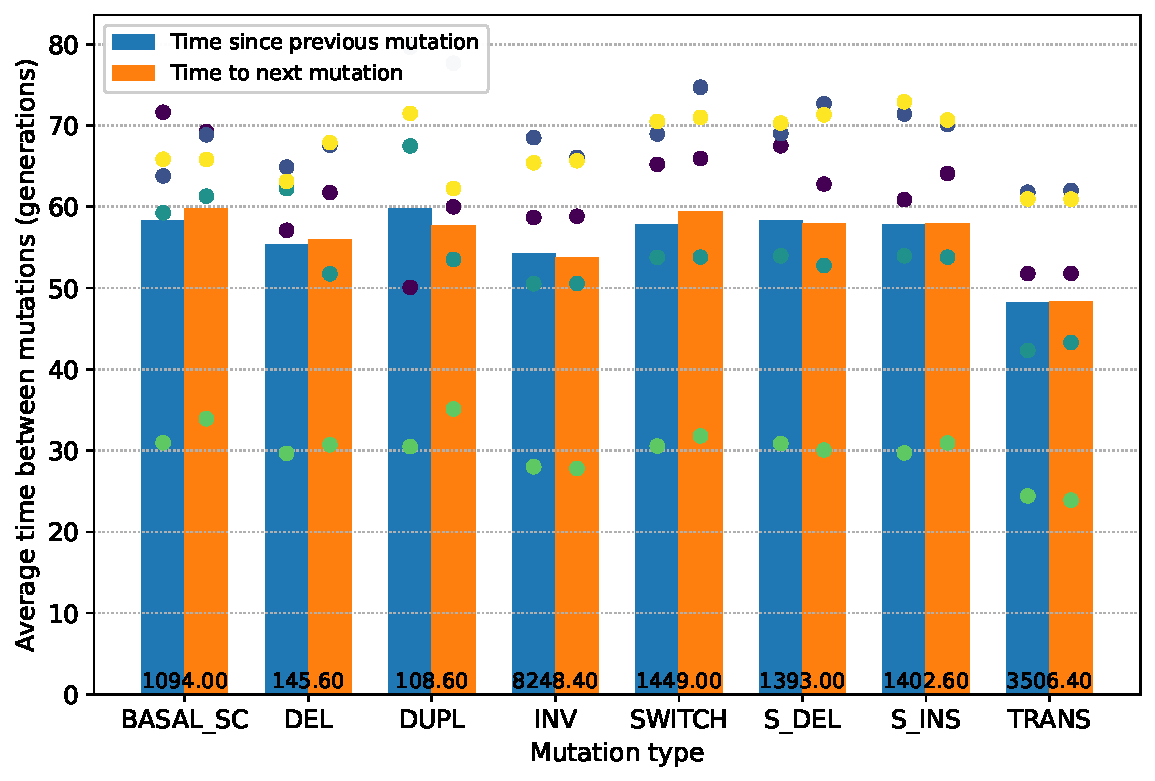
\includegraphics[width=\textwidth]{aevol/images/with_sc_mut_time_150k_995k.pdf}
\caption{I need to remember the mutation types}
\end{figure}


\section{Conclusion}
\label{sec:aevol:ccl}